\documentclass{article}
\usepackage[left=25mm,right=25mm,bottom=35mm]{geometry}
\usepackage{amsmath,graphicx}
\usepackage[comma,numbers,square,sort&compress]{natbib}

\begin{document}

\title{Fault diagnosis method of pitch actuators for wind turbines based on variable forgetting factor identification algorithm}

\author{Dinghui WU,
        Zhicheng JI}
\date{}
\maketitle


\begin{abstract}
To diagnose the fault in pitch actuator of wind turbines, a fault diagnosis method is proposed
in this paper, which is based on the variable forgetting factor recursive least-squares
algorithm. According to the characteristic that the system parameters are changed by faults,
the VFF-RLS system identification algorithm is adopted to estimate the changing
parameters. The fault diagnosis problem is transformed into a parameter estimation
issue. Then the time-varying natural frequency and damping ratio of pitch actuators
are estimated based on the discrete model. The convergence rate and identification accuracy of the
identification algorithm can be guaranteed by adjusting the forgetting factor automatically.
The simulation results validate the effectiveness of the proposed method.
\end{abstract}

\textbf{Keywords: wind turbines; pitch actuator; fault diagnosis; system identification; variable forgetting factor}

\footnotetext{\\
Key laboratory of Advanced Process Control for Light Industry, Ministry of Education, Jiangnan University, Wuxi, 214122, China\\
Corresponding author:\\
Dinghui Wu, Key laboratory of Advanced Process Control for Light Industry, Ministry of Education, Jiangnan University, Wuxi 214122, China\\
Email: wh033098@163.com\\
This research was supported by Prospective Joint Research Project of Industry, Education and Academy of Jiangsu Province (BY2012071) and China Postdoctoral Science Foundation (2013M531272).}




\section{Introduction}

As the fastest growing renewable energy, the wind energy has raised
the world's attention \cite{ref:1}. But wind farms are generally built
in adverse conditions such as desert or sea areas \cite{ref:2}, which
may cause severe failures. The hydraulic pitch systems adjusts the pitch angle
for constant power output, while wind speed is higher than the rated value,
is an important component of the pitch wind turbine \cite{ref:3}.
Once it fails, it directly affects the system stability, so accurate fault
diagnosis for pitch wind turbine is essential.

Hydraulic pitch system fault diagnosis method is broadly divided into two
categories, which is based on the data-driven, the model and the data-driven
approach, Crowther  uses neural networks for fault diagnosis of
the hydraulic system \cite{ref:4}. Goharrizi uses Hilbert transform on fault detection of hydraulic actuator hydraulic leaks \cite{ref:5}.

Goharrizi uses the fast Fourier transform and Wavelet transform method for detection
of actuator hydraulic leaks \cite{ref:6}. However, the data-driven based approach
 often requires a lot of prior knowledge about the failure characteristics.
Model-based methods without prior knowledge, has got more attention and development
\cite{ref:7}. For the wind turbine pitch system, Wei uses the filter and observer to
diagnose pitch actuator fault \cite{ref:8}. Wu uses the adaptive parameter
estimation algorithm which is based on dynamic model of hydraulic pitch system, to
detect the pitch system hydraulic pressure leakage fault \cite{ref:9}.

The system identification method uses the system's input and output data to estimate
parameters \cite{ref:10}. When hydraulic pitch system fails, some
parameters of the pitch change, system identification methods can be used to estimate the change of data, and the fault diagnosis problem can
be converted to the parameter estimation \cite{ref:11}. Faulty pitch
systems can be modeled as a time-varying system, and a forgetting factor
is introduced to  estimates the time-varying system effectively.
But identification methods of time-varying parameter with forgetting factor cannot achieve
satisfactory result. While the forgetting factor is large, the algorithm converges slowly,
while the forgetting factor is small, the algorithm produces large estimation errors \cite{ref:12}.
Identification algorithm with variable forgetting factor can automatically choose
a appropriate forgotten
factor, to achieve high convergence speed and accuracy \cite{ref:13}. Therefore, this
paper utilizes the variable forgetting factor recursive least squares (VFF-RLS)
identification algorithms to estimate parameters of pitch system, the
estimated values are
compared with theoretical value to detect faults and identify the fault type.


\section{Model Description}


\subsection{Wind Turbine Model}

The wind turbine system includes the aerodynamic subsystem, the pitch subsystem, the drive train
subsystem and the power subsystem. Among them, the power subsystem is consisted of the
generator and converter. The interconnected relationship of various subsystem is
shown in Fig. \ref{fig:1} \cite{ref:14}.

\begin{figure}[!htb]
  \centering
  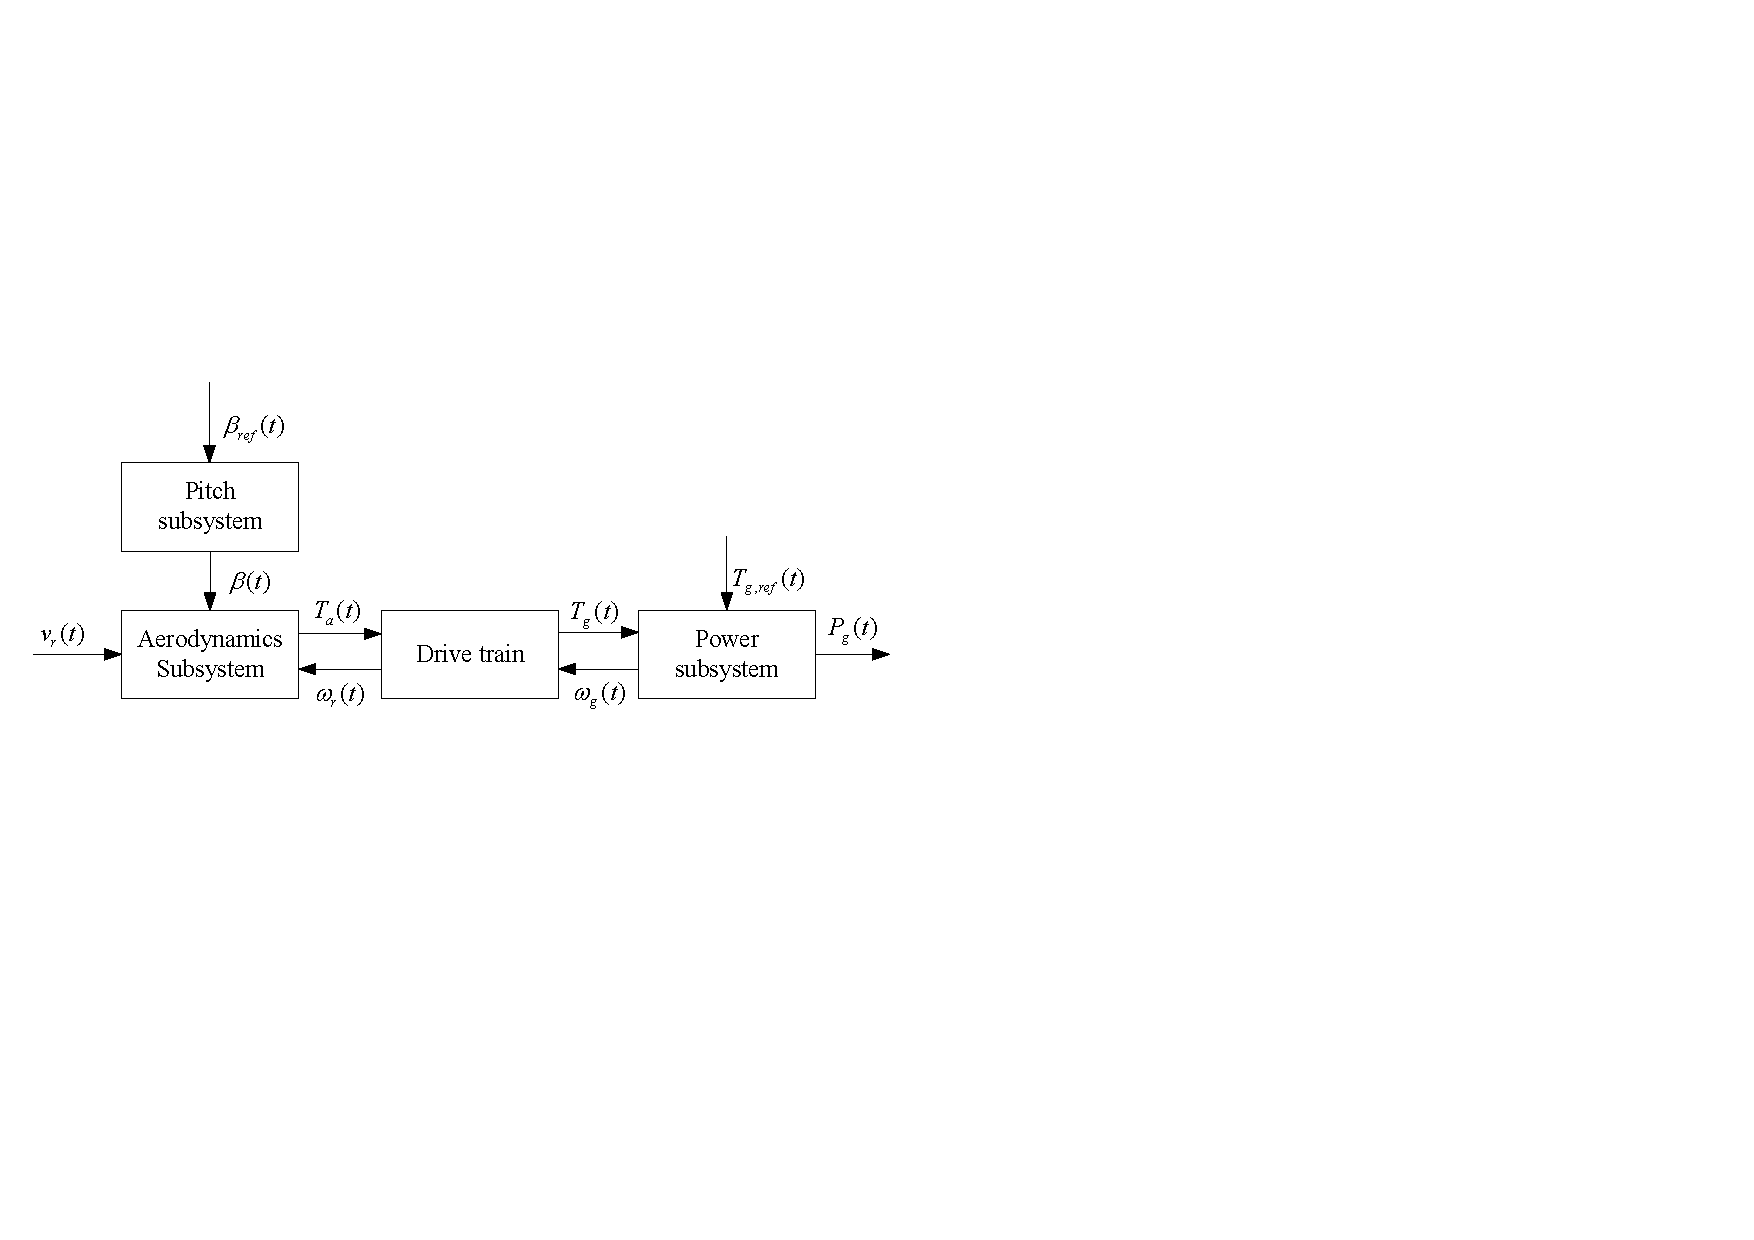
\includegraphics[]{fig1.pdf}
  \caption{The structure of the wind turbine system model}
  \label{fig:1}
\end{figure}


The aerodynamic subsystem produces aerodynamic torque under the action of
the effective wind speed $v_r(t)$, the rotor speed $\omega_r(t)$ and
the pitch angle $\beta(t)$. The drive train subsystem transmits the rotor speed  $\omega_r(t)$
to the generator speed $\omega_g(t)$. The electrical power generated by the
converter is connected to the public power grid.
For variable pitch wind turbines, in order to meet the operational requirements
of the variable speed variable pitch, blade pitch angle $\beta(t)$ and torque $T_g(t)$
are adjusted according to  the reference value $\beta_{ref}(t)$ and $T_{g,ref}(t)$.
The pitch angle $\beta(t)$ is controlled by the pitch system, and the torque $T_g(t)$
is controlled by
the converter.



\subsection{Pitch and Fault Model}


The wind turbine hydraulic pitch system schematic is shown in Fig. \ref{fig:2},
it contains: 1. the hydraulic pump, 2. the hydraulic tank,
3. the proportioning valve, 4. the safety valve,
5. the hydraulic actuator and 6. the
slider-crank mechanism. The crank-slider mechanism
is used to connect the pitch by pitch actuators, the pitch angle is adjusted by
rotating blades.

\begin{figure}[!htb]
  \centering
  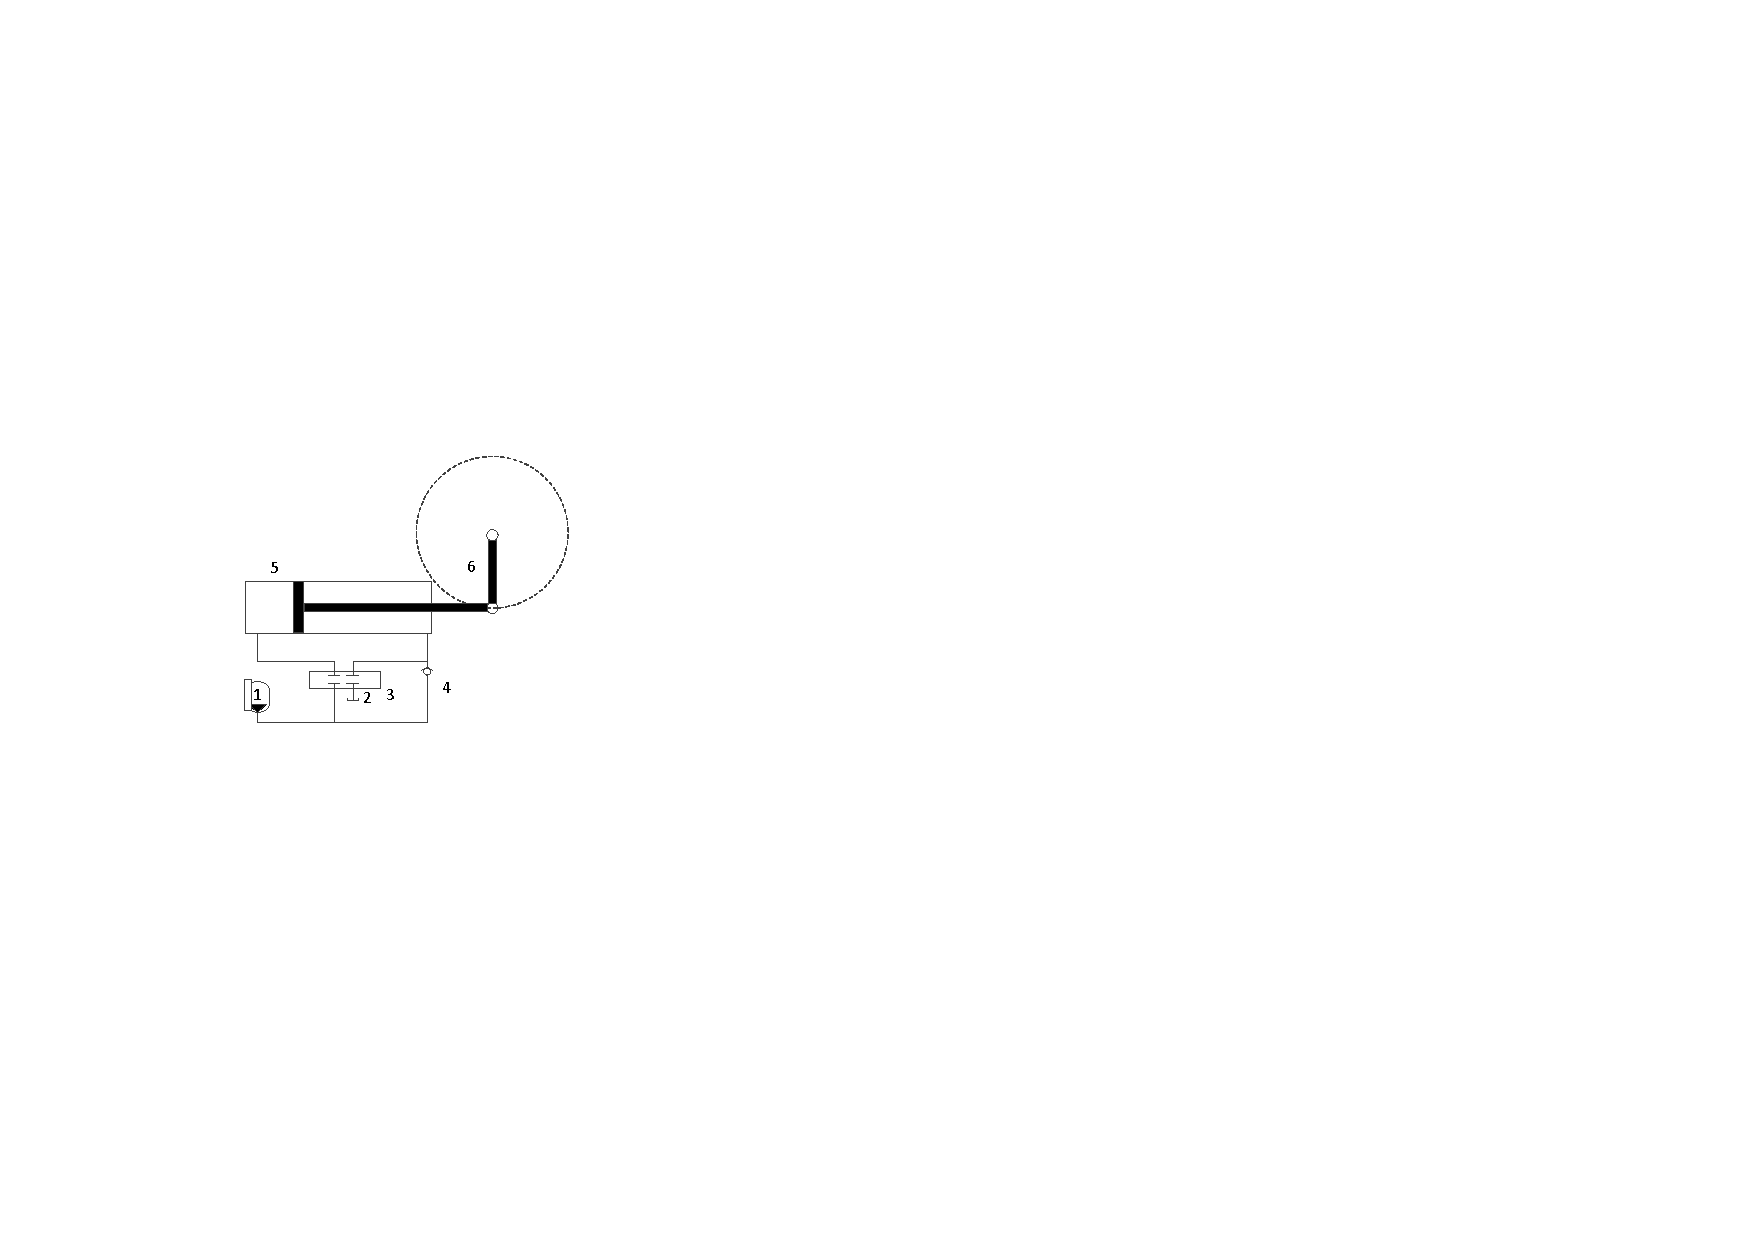
\includegraphics[]{fig2.pdf}
  \caption{The hydraulic pitching system}
  \label{fig:2}
\end{figure}

The hydraulic pitch actuator can be modeled as a second order system \cite{ref:15},
the dynamic model is
\begin{eqnarray}
  \ddot{\beta}(t) = -2\zeta\omega_n\dot{\beta}(t) - \omega^2_n\beta(t) + \omega^2_n\beta_{ref}(t),
\end{eqnarray}
where $\omega_n$ is the natural frequency of actuator, $\zeta$ is the damping ratio.
of the actuator.

This paper focuses on the following pitch faults,
the high air content in the hydraulic oil, the hydraulic leakage and the pump wear.
Faults affect the dynamic properties of the system by changing the  natural frequency and
the damping coefficient.
Under the influence of the fault, the natural frequency and the damping coefficient
changes from the nominal value $\omega_{n,0}$ and $\zeta_0$to three kinds of parameter values,
which is $\omega_{n,ha}$ and $\zeta_{ha}$, $\omega_{n,hl}$ and $\zeta_{hl}$, $\omega_{n,pw}$ and $\zeta_{pw}$.

The dynamic model of the pitch system with fault is
\begin{eqnarray}
  \ddot{\beta}(t) = -2\zeta(t)\omega_n(t)\dot{\beta}(t) - \omega^2_n(t)\beta(t) + \omega^2_n(t)\beta_{ref}(t),   \label{eq:2}
\end{eqnarray}
where $\zeta(t)$ and $\omega_n(t)$ have different values under different faults, the specific
expression is
\begin{eqnarray}
  \omega_n(t) &=& (1-\eta_{ha}(t))\omega_{n,0}  + \eta_{ha}(t)\omega_{n,ha},    \label{eq:3}\\
  \zeta(t)    &=& (1-\eta_{ha}(t))\zeta_0       + \eta_{ha}(t)\zeta_{ha},       \label{eq:4}\\
  \omega_n(t) &=& (1-\eta_{hl}(t))\omega_{n,0}  + \eta_{hl}(t)\omega_{n,hl},    \label{eq:5}\\
  \zeta(t)    &=& (1-\eta_{hl}(t))\zeta_0       + \eta_{hl}(t)\zeta_{hl},       \label{eq:6}\\
  \omega_n(t) &=& (1-\eta_{pw}(t))\omega_{n,0}  + \eta_{ha}(t)\omega_{n,pw},    \label{eq:7}\\
  \zeta(t)    &=& (1-\eta_{pw}(t))\zeta_0       + \eta_{ha}(t)\zeta_{pw},       \label{eq:8}
\end{eqnarray}
where $\eta_{ha}(t)$, $\eta_{hl}(t)$ and $\eta_{pw}(t)$ are the indicator of the
high air content in the hydraulic oil, the hydraulic leakage and the pump wear, and
$0\leq\eta_{ha}(t)\leq1, 0\leq\eta_{hl}(t)\leq1, 0\leq\eta_{pw}(t)\leq1$.







\section{Fault Diagnosis Method Based on VFF-RLS }

\subsection{Structure of the Fault Diagnosis System}

Based on the pitch actuator fault model, the VFF-RLS algorithm is used to
diagnose faults. Fault diagnosis method needs the input
and output data of the pitch system. The method take the pitch angle reference $\beta_{ref}(t)$
as the input of the algorithm,
and the actual pitch angle
as the output of the algorithm.  The pitch actuator
parameters $\omega_n(t)$ and $\zeta(t)$ can be estimated through the VFF-RLS algorithm.

From the Eq.(\ref{eq:3}) to Eq.(\ref{eq:8}),  the
natural frequency $\omega_n(t)$ and the damping coefficient $\zeta(t)$ of each kind of
fault have the corresponding curve with the signal $\eta(t)$.
It is assumed in this paper that two or more faults will not occur simultaneously, the
identification estimates two parameter values on their respective curves,
when $\eta(t)$ is greater than a certain threshold, it indicates a fault has occurred.
Then, according to estimated values $\omega_n(t)$ and $\zeta(t)$ the corresponding
curve is determined, thereby
the distinguish of the fault type can be completed. The structure of fault diagnosis
is shown in Fig. \ref{fig:3}.

\begin{figure}[!htb]
  \centering
  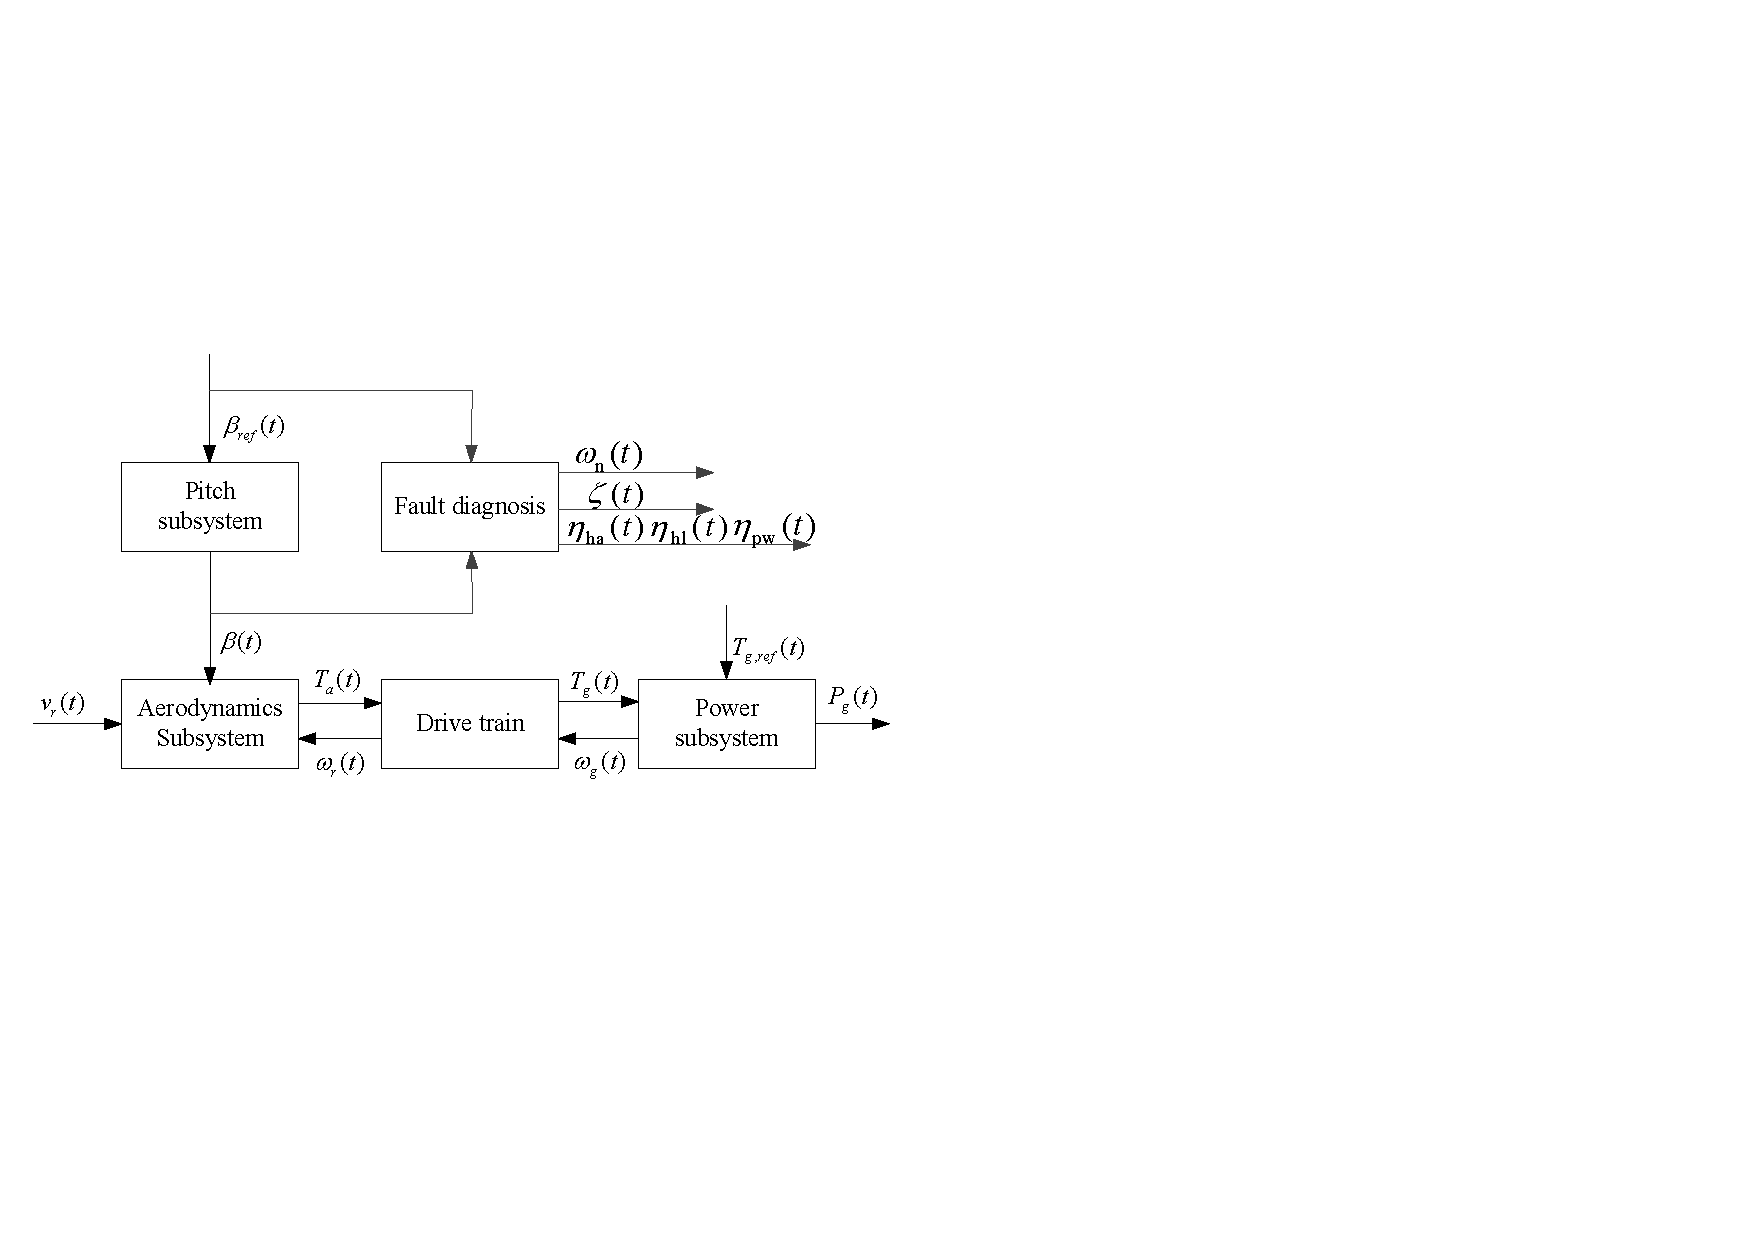
\includegraphics[]{fig3.pdf}
  \caption{The structure chart for fault diagnosis}
  \label{fig:3}
\end{figure}


\subsection{Discrete Model}

The system identification algorithm must be implemented by a computer program,
so the model needs to be discretization from the continuous system model, and
eventually be converted into the corresponding difference equation.

First of all, for the pitch system with fault depicted in Eq.(\ref{eq:2}),
$x(t)=[\beta(t), \dot{\beta(t)}]^\mathrm{T}$ is chosen as the state variables,
$y(t)=\beta(t)$ is chosen as the output, its normative state space equation for
the continuous system is
\begin{eqnarray}
  \left\{\begin{aligned}
    \dot{x}(t) &=& \bar{A}x(t) &+ \bar{B}u(t)  \\
    y(t)       &=& \bar{C}x(t) &
  \end{aligned},
  \right.                    \label{eq:9}
\end{eqnarray}
where $\bar{A}=\begin{bmatrix}
  0              & 1                      \\
  -\omega^2_n(t) & -2\zeta(t)\omega_n(t)
\end{bmatrix}^\mathrm{T}$,
$\bar{B}=\begin{bmatrix}
  0 & \omega^2_n(t)
\end{bmatrix}^\mathrm{T}$,
$\bar{C}=\begin{bmatrix}
  1 & 0
\end{bmatrix}$.


Then, the discrete model is obtained from the continuous-time state equation.
The impulse invariant transformation
method is commonly used discretization, which can ensure the output of the discrete model
is equal to output of
the continuous-time system at certain
sample points \cite{ref:16}. Take the sampling period as $T_0$, when the period is
small, the $u(t)$ can be considered unchanged during one sampling period, that is
$u(t)=u(kT_0), kT_0\leq{}t<(k+1)T_0$. We denote $x(kT_0)=:x(k),u(kT_0)=:u(k),y(kT_0):=y(k)$,
then the discrete model from Eq.(\ref{eq:9}) is
\begin{eqnarray}
  \left\{\begin{aligned}
    x(k+1)     &=& Ax(k) &+ Bu(k)  \\
    y(k)       &=& Cx(k) &
  \end{aligned},
  \right.                    \label{eq:10}
\end{eqnarray}
where $A=e^{\bar{A}T_0} \approx I+\bar{A}T_0 =
\begin{bmatrix}
  1                   &    T_0      \\
  -\omega^2_n(k)T_0   &    1-2\zeta(k)\omega_n(k)T_0
\end{bmatrix}$,
$B=
\begin{bmatrix}
  \int{}e^{\bar{A}(T_0-t)}dt
\end{bmatrix}\bar{B}=\bar{B}T_0=
\begin{bmatrix}
  0    &  \omega^2_n(k)T_0
\end{bmatrix}^\mathrm{T}$,
$C=\bar{C}=
\begin{bmatrix}
  1  &   0
\end{bmatrix}$.



\subsection{Analysis of the System Parameter's identifiablity}

System identification methods can only be used in the identifiable
system. As this paper identifies changing parameters of the system,
it is necessary to determine whether the system is a parameter
identifiable system. According to the Eq.(\ref{eq:10}),
the controllability matrix of the system is
$Q_e=
\begin{bmatrix}
  B   &   AB
\end{bmatrix}=
\begin{bmatrix}
  0             &   \omega^2_n(k)T^2_0   \\
  \omega^2_n(k) &   (1-2\zeta(k)\omega_n(k)T_0)\omega^2_n(k)T_0
\end{bmatrix}$,
$rank{}Q_e=2$, the controllability matrix is full rank, so the system
can be controlled. The system observability matrix is
$$Q_o =
\begin{bmatrix}
  C \\
  CA
\end{bmatrix} =
\begin{bmatrix}
  1  &  0  \\
  1  &  T_0
\end{bmatrix}$$,
$rank{}Q_o=2$, the observability matrix is full rank, so the system can
be observed. From the above analysis, this system is a identifiable.


The system's input and output expressions are
\begin{eqnarray}
  y(k) &=& C(zI-A)^{-1}B{}u(k)   \notag\\
       &=& b_2(k)z^{-2}u(k)/1 + a_1(k)z^{-1} + a_2(k)z^{-2} \label{eq:11}
\end{eqnarray}
where $a_1(k), a_2(k)$ and $b_2(k)$ are
\begin{eqnarray}
  a_1(k) &=&  2\zeta(k)\omega_n(k)T_0-2    \label{eq:12}\\
  a_2(k) &=&  \omega^2_n(k)T^2_0 + 1 - 2\zeta(k)\omega_n(k)T_0 \label{eq:13} \\
  b_2(k) &=&  \omega^2_n(k)T^2_0 \label{eq:14}
\end{eqnarray}

Eq.(\ref{eq:11}) can be written as a differential equation
\begin{eqnarray}
  y(k) + a_1(k)y(k-1) + a_2(k)y(k-2) = \notag\\
  b_2(k)u(k-2) + v(k)            \label{eq:15}
\end{eqnarray}

The system identification algorithm is able to estimate the
coefficients $a_1(k)$, $a_2(k)$ and $b_2(k)$. The time-varying parameters
$\zeta$ and $\omega_n(k)$ can be obtained from the Eq.(\ref{eq:12}) to
Eq.(\ref{eq:14}), and the system Eq.(\ref{eq:10}) is parameter
identifiable. Therefore, system identification methods can be used to
estimate the wind turbine system.

\subsection{Fault Diagnosis Algorithm}

The VFF-RLS algorithm is based on the identification model, which
consisted of the discrete systems Eq.(\ref{eq:10}) and
the differential equation Eq.(\ref{eq:15}),
\begin{eqnarray}
  y(k) = \varphi^\mathrm{T}(k)\theta + v(k)   \label{eq:16}
\end{eqnarray}
where $\varphi(k)=
\begin{bmatrix}
  -y(k-1)  &  -y(k-2)   &   -u(k-2)
\end{bmatrix}^\mathrm{T}$ is the information vector,
$\theta(k) =
\begin{bmatrix}
  a_1(k)   &   a_2(k)   &   b_2(k)
\end{bmatrix}^\mathrm{T}$ is the parameters to be estimated,
$v(k)$ is the white noise with zero mean.

The estimated value of the identification model Eq.(\ref{eq:16}) can
be obtained from VFF-RLS algorithm defined by the following equation,
\begin{eqnarray}
  d(k)            & = & y(k) - \varphi^\mathrm{T}(k)\hat{\theta}(k-1),   \label{eq:17}\\
  L(k)            & = & \frac{P(k-1)\varphi(k)}{\lambda(k)+\varphi^\mathrm{T}(k)P(k-1)\varphi(k)},  \label{eq:18}\\
  \hat{\theta}(k) & = & \hat{\theta}(k-1) + L(k)d(k),  \label{eq:19}  \\
  P(k)            & = & \frac{1}{\lambda(k)}[P(k-1) - L(k)\varphi^\mathrm{T}(k)P(k-1)],
\end{eqnarray}
where $\lambda(k)$ is the variable forgetting factor, $L(k)$ is the
gain matrix, $P(k)$ is the covariance matrix.

As the $k-1$ estimator is used by the parameter $d(k)$ of
the Eq.(\ref{eq:17}), it is a priori error. The posteriori error is
defined as
\begin{eqnarray}
  \mu(k) = y(k) - \varphi^\mathrm{T}(k)\hat{\theta}(k)   \label{eq:21}
\end{eqnarray}
combined with the Eq.(\ref{eq:17}), Eq.(\ref{eq:18}) and Eq.(\ref{eq:19}),
the Eq.(\ref{eq:21}) can be converted to
\begin{eqnarray}
  \mu(k) = d(k)\begin{bmatrix}
  1-\frac{\varphi^\mathrm{T}(k)P(k-1)\varphi(k)}{\lambda(k)+\varphi^\mathrm{T}P(k-1)\varphi{k}}]
  \end{bmatrix}, \label{eq:22}
\end{eqnarray}
we denote $h(k) = \varphi^\mathrm{T}P(k-1)\varphi(k)$, so
\begin{eqnarray}
  \mu(k) = d(k)\begin{bmatrix}
    1-\frac{h(k)}{\lambda(k) + h(k)}
  \end{bmatrix}.   \label{eq:23}
\end{eqnarray}

The variance of the system noise $v(k)$ is $\sigma$, a posteriori error
covariance is approximately equal to the noise variance, that is
$E[\mu^2(k)]=\sigma^2_v(k)$, $E$ is the expectation operator.
Combined with Eq.(\ref{eq:23}),
\begin{eqnarray}
  E\left\{d^2(k)\begin{bmatrix}
    1-\frac{h(k)}{\lambda(k)+h(k)}
  \end{bmatrix}^2\right\}=\sigma^2_v(k), \label{eq:24}
\end{eqnarray}
where $E[d^2(k)]=\sigma^2_d(k), E[h^2(k)]=\sigma^2_v(k)$.

However, the variance $\sigma^2_v(k)$, $\sigma^2_d(k)$ and $\sigma^2_h(k)$
is difficult to get an accurate value,
the $\hat{\sigma}^2_v(k)$,  $\hat{\sigma}^2_d(k)$ and
$\hat{\sigma}^2_h(k)$ can be obtained based on the estimated
variance in length of the data collected, which are
\begin{eqnarray}
  \hat{\sigma}^2_v(k)      & = & \frac{1}{k}\sum^k_{j=1}[y(j) - \varphi^\mathrm{T}(j)\hat{\theta}(j)]^2     \\
  \hat{\sigma}^2_d(k)      & = & \frac{1}{k}\sum^k_{j=1}[y(j) - \varphi^\mathrm{T}(j)\hat{\theta}(j-1)]^2   \\
  \hat{\sigma}^2_h(k)      & = & \frac{1}{k}\sum^k_{j=1}[\varphi^\mathrm{T}(j)P(j-1)\varphi(j)]^2  \label{eq:27}
\end{eqnarray}
By solving the Eq.(\ref{eq:24}), the variable forgetting factor
$\lambda(k)$ is
\begin{eqnarray}
  \lambda(k) = \frac{\sigma_h(k)\sigma_v(k)}{\sigma_d(k)-\sigma_v(k)} \label{eq:28}
\end{eqnarray}

As the forgotten factor $\lambda$ is greater than zero, in
Eq.(\ref{eq:28}), $\sigma_d(k)\geq\sigma_v(k)$.
It is obviously when $\hat{\sigma}_d(k)\leq\hat{\sigma}_v(k)$, we
can set $\lambda(k)=\lambda_{min}$. However, when the algorithm is
in a stable state, the value of $\hat{\sigma}_d(k)$ fluctuate around
the value of $\hat{\sigma}_v(k)$, this limits
the above setting method. More appropriate approach needs to be
chosen, that is when $\hat{\sigma}_d(k)\leq\gamma\hat{\sigma}_v(k)(1<\gamma<2)$,
 sets $\lambda(k)=\lambda_{min}$, $\lambda_{min}$ is taken as a
value which is close or equal to 1. Otherwise, the forgetting
factor of the VFF-RLS algorithm will
automatically adjusted to
\begin{eqnarray}
  \lambda(k)=min\left\{
  \frac{\sigma_h(k)\sigma_v(k)}{\xi+\sigma_d(k) - \sigma_v(k)}, \lambda_{max}\right\}.     \label{eq:29}
\end{eqnarray}

In order to prevent the denominator to be zero, $\xi$ in
Eq.(\ref{eq:29}) is taken as the minimum value, and the $\xi$
is the minimum positive constant.
When the system changes, $\hat{\sigma}_d(k)$ is significantly greater
than $\hat{\sigma}_v(k)$, the forgetting factor $\lambda$ in Eq.(\ref{eq:29})
is automatically switched to the smaller value to
increase the convergence speed.
When the algorithm tends to converge into a stable state, the
$\hat{\sigma}^2_d(k) \cong \hat{\sigma}^2_v(k)$, and meet
$\hat{\sigma}_d(k) \leq \hat{\sigma}_v(k)$, $\lambda(k)$ should become
$\lambda_{max}$ to reduce estimate errors and improve identification
accuracy.


\begin{figure}[!htb]
  \centering
  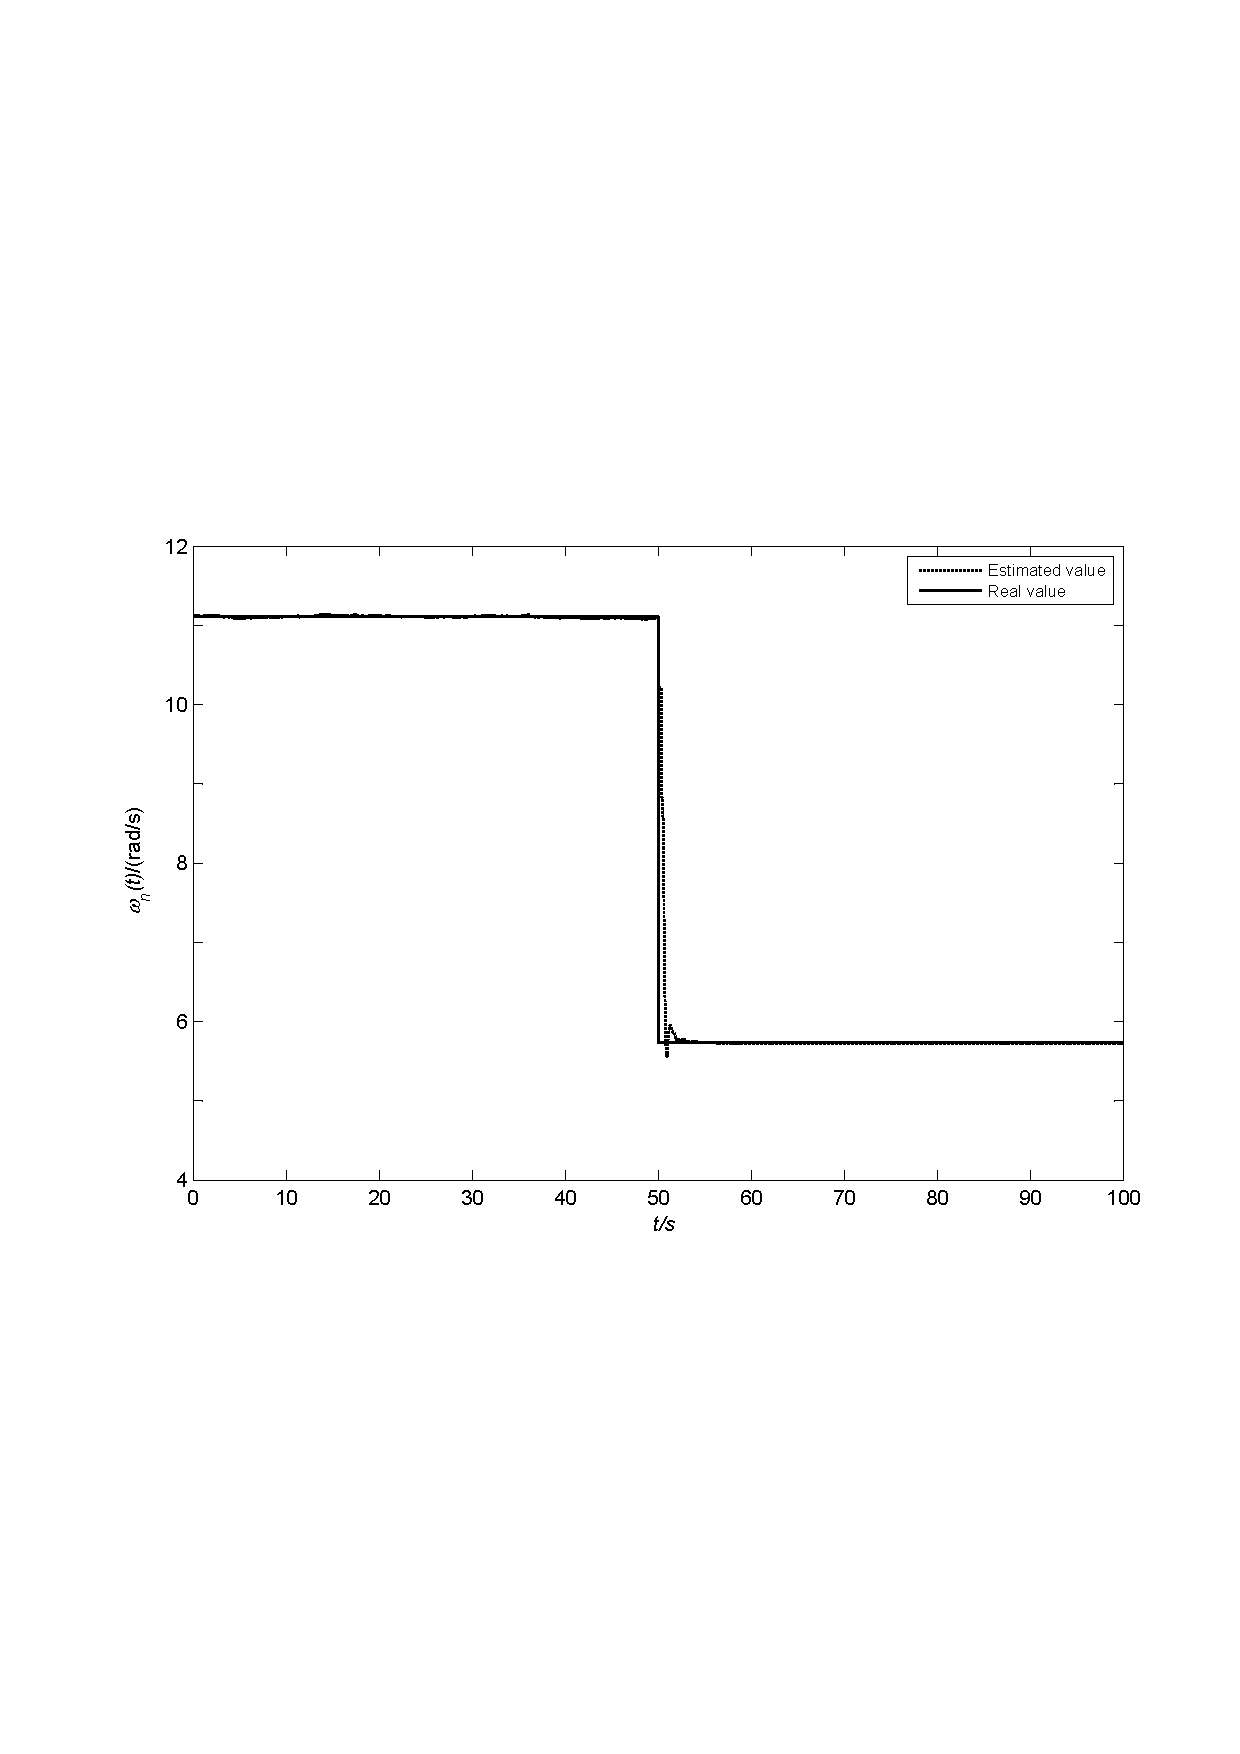
\includegraphics[width=\hsize]{fig4a.pdf}
  \caption{The parameter $\omega_n(t)$ of the high air content in the hydraulic oil}
  \label{fig:4}
\end{figure}


\begin{figure}[!htb]
  \centering
  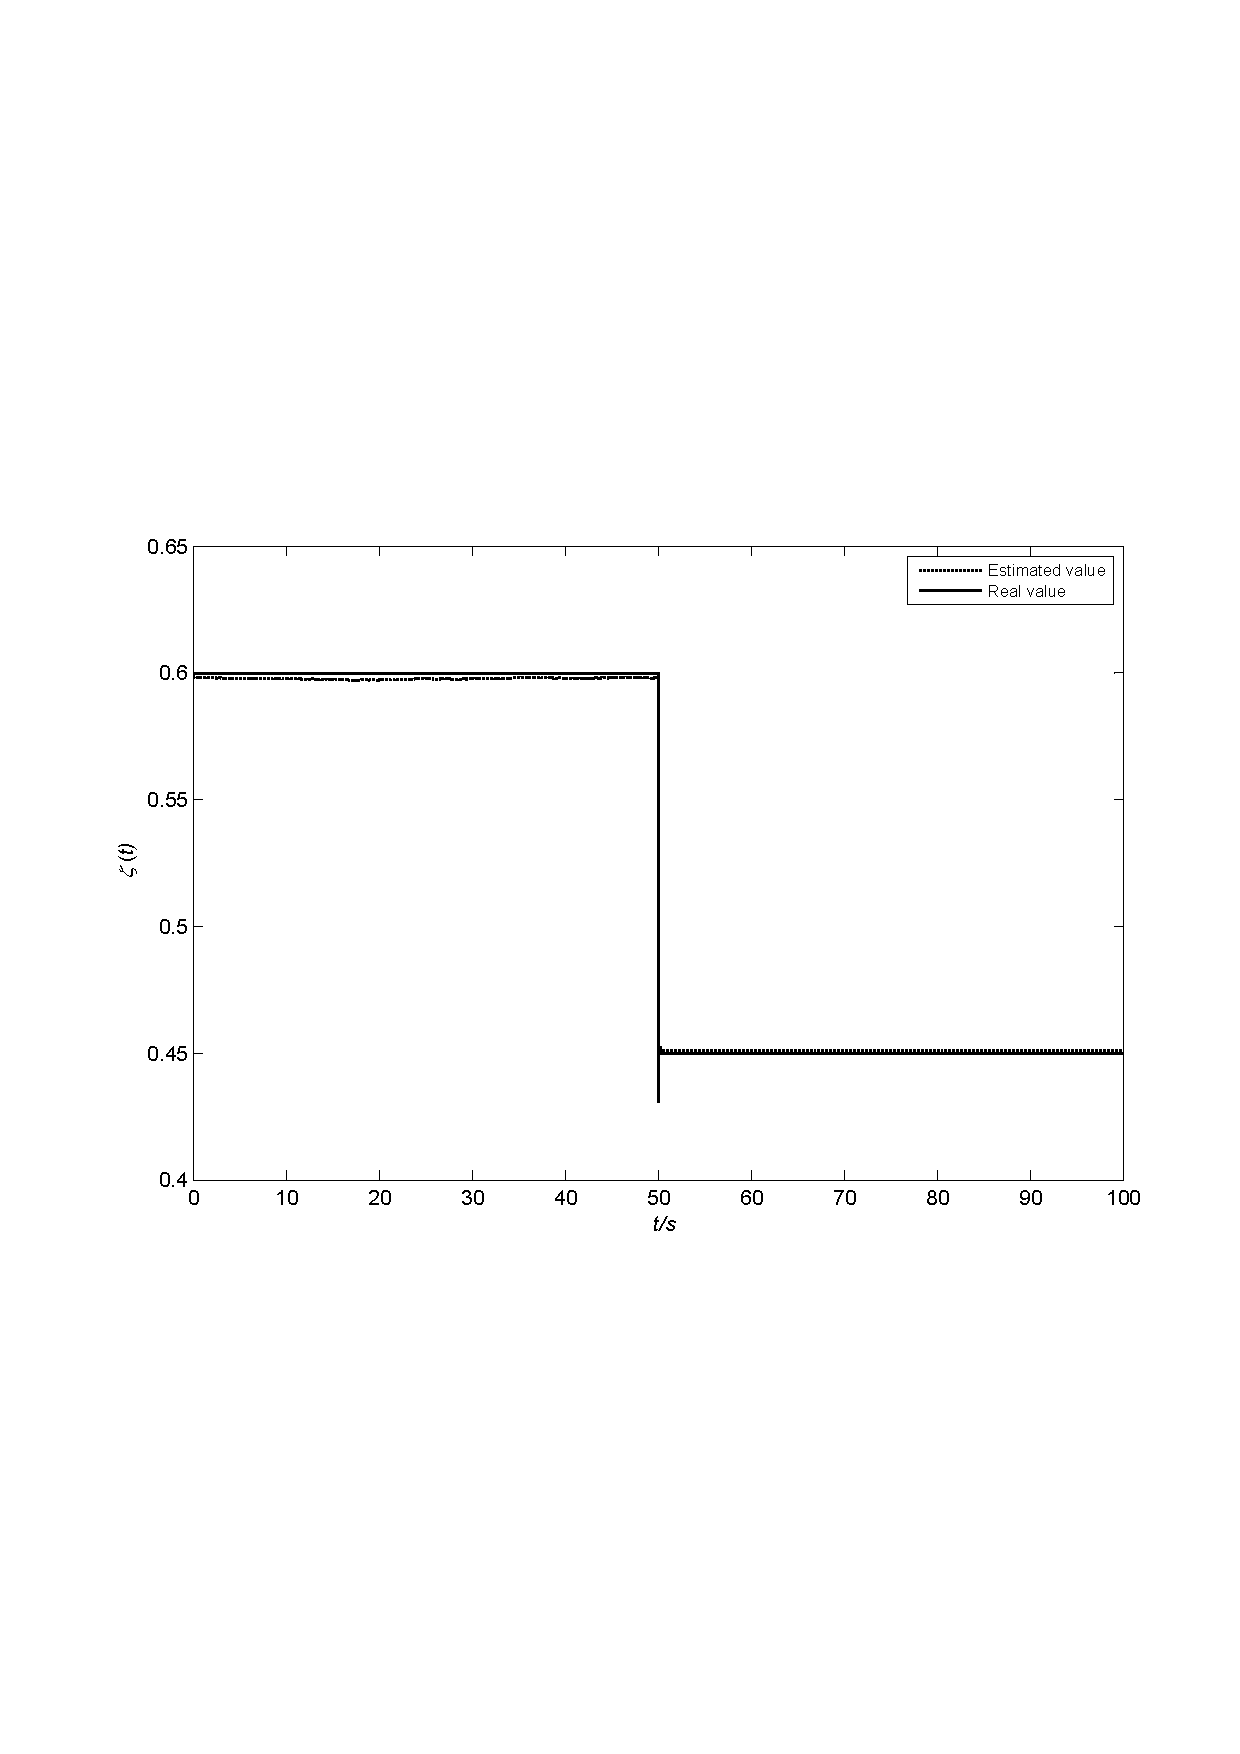
\includegraphics[width=\hsize]{fig4b.pdf}
  \caption{The parameter $\zeta(t)$ of the high air content in the hydraulic oil}
  \label{fig:4b}
\end{figure}


\begin{figure}[!htb]
  \centering
  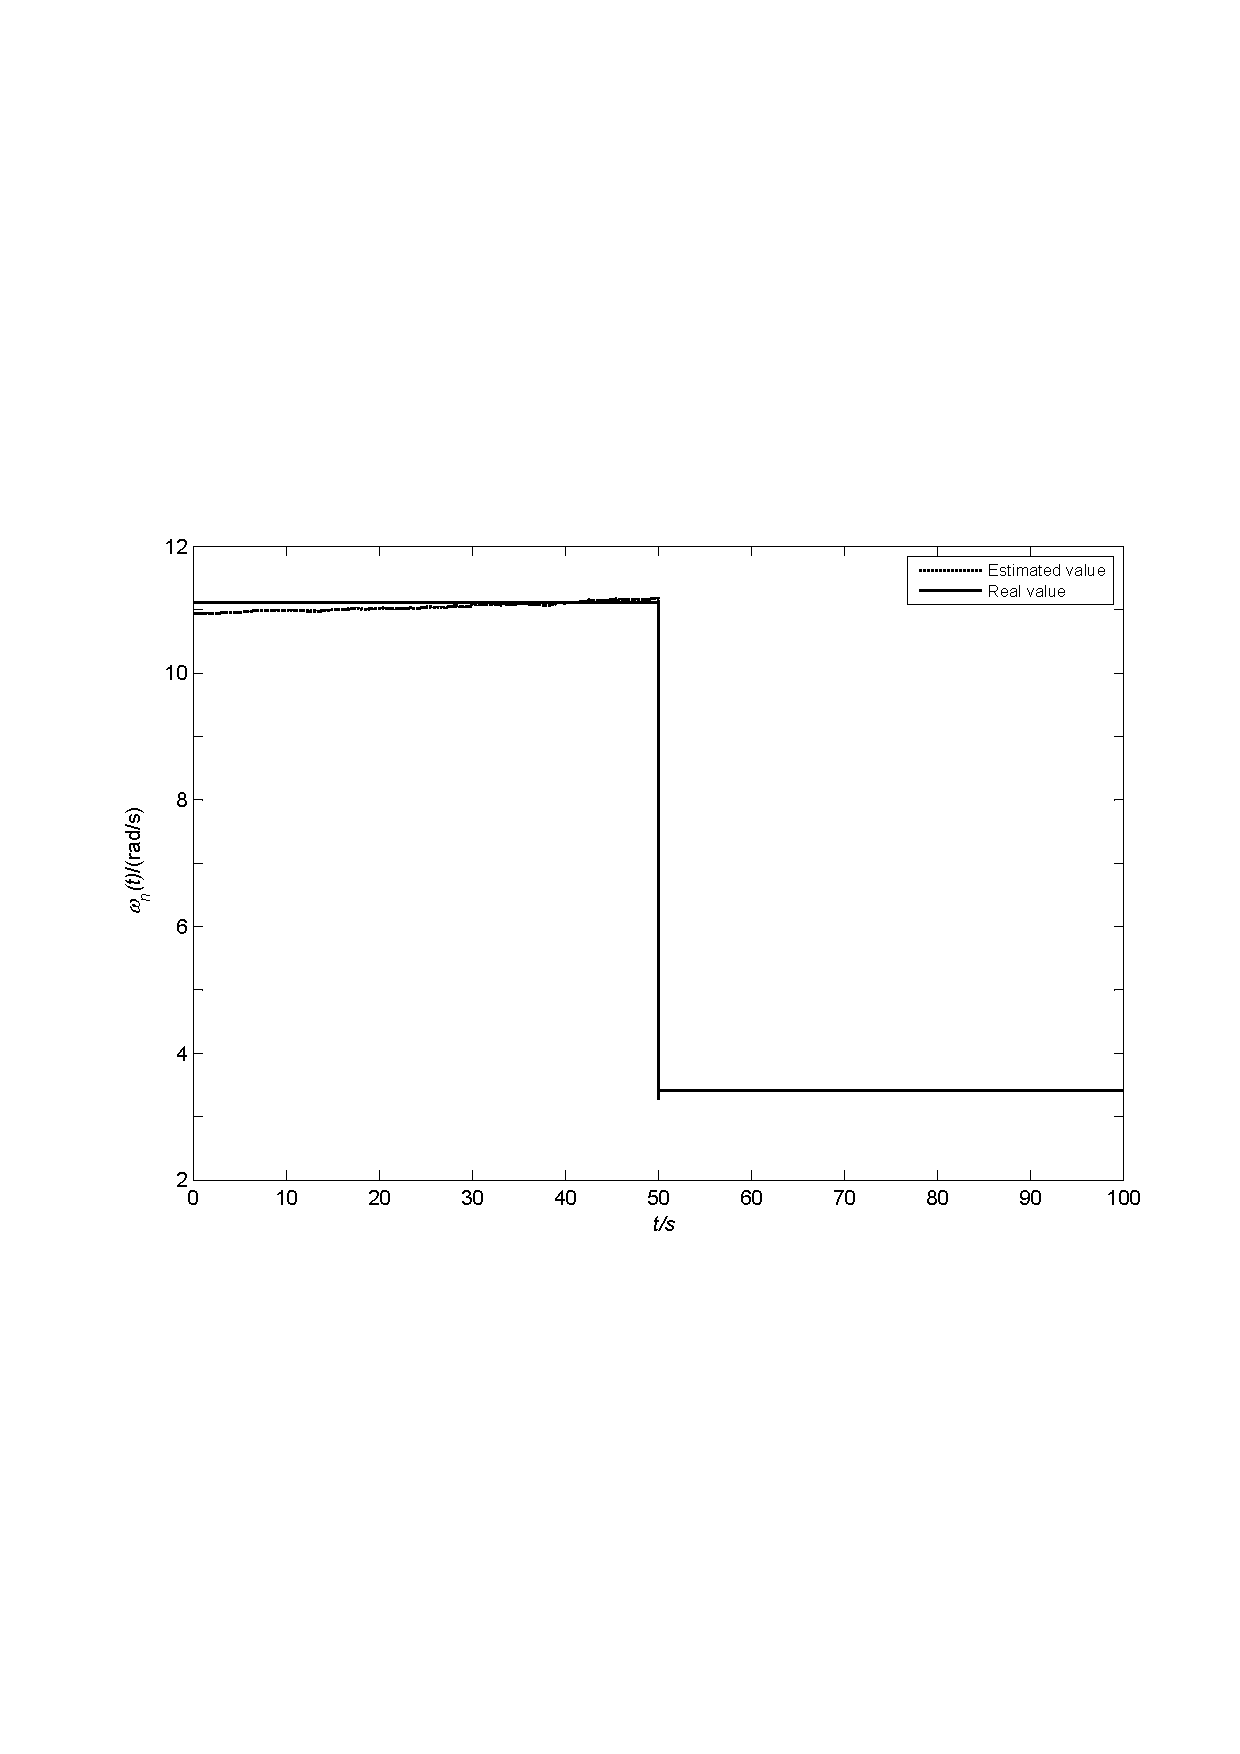
\includegraphics[width=\hsize]{fig5a.pdf}
  \caption{The parameter $\omega_n(t)$ of hydraulic leakage}
  \label{fig:5}
\end{figure}


\begin{figure}[!htb]
  \centering
  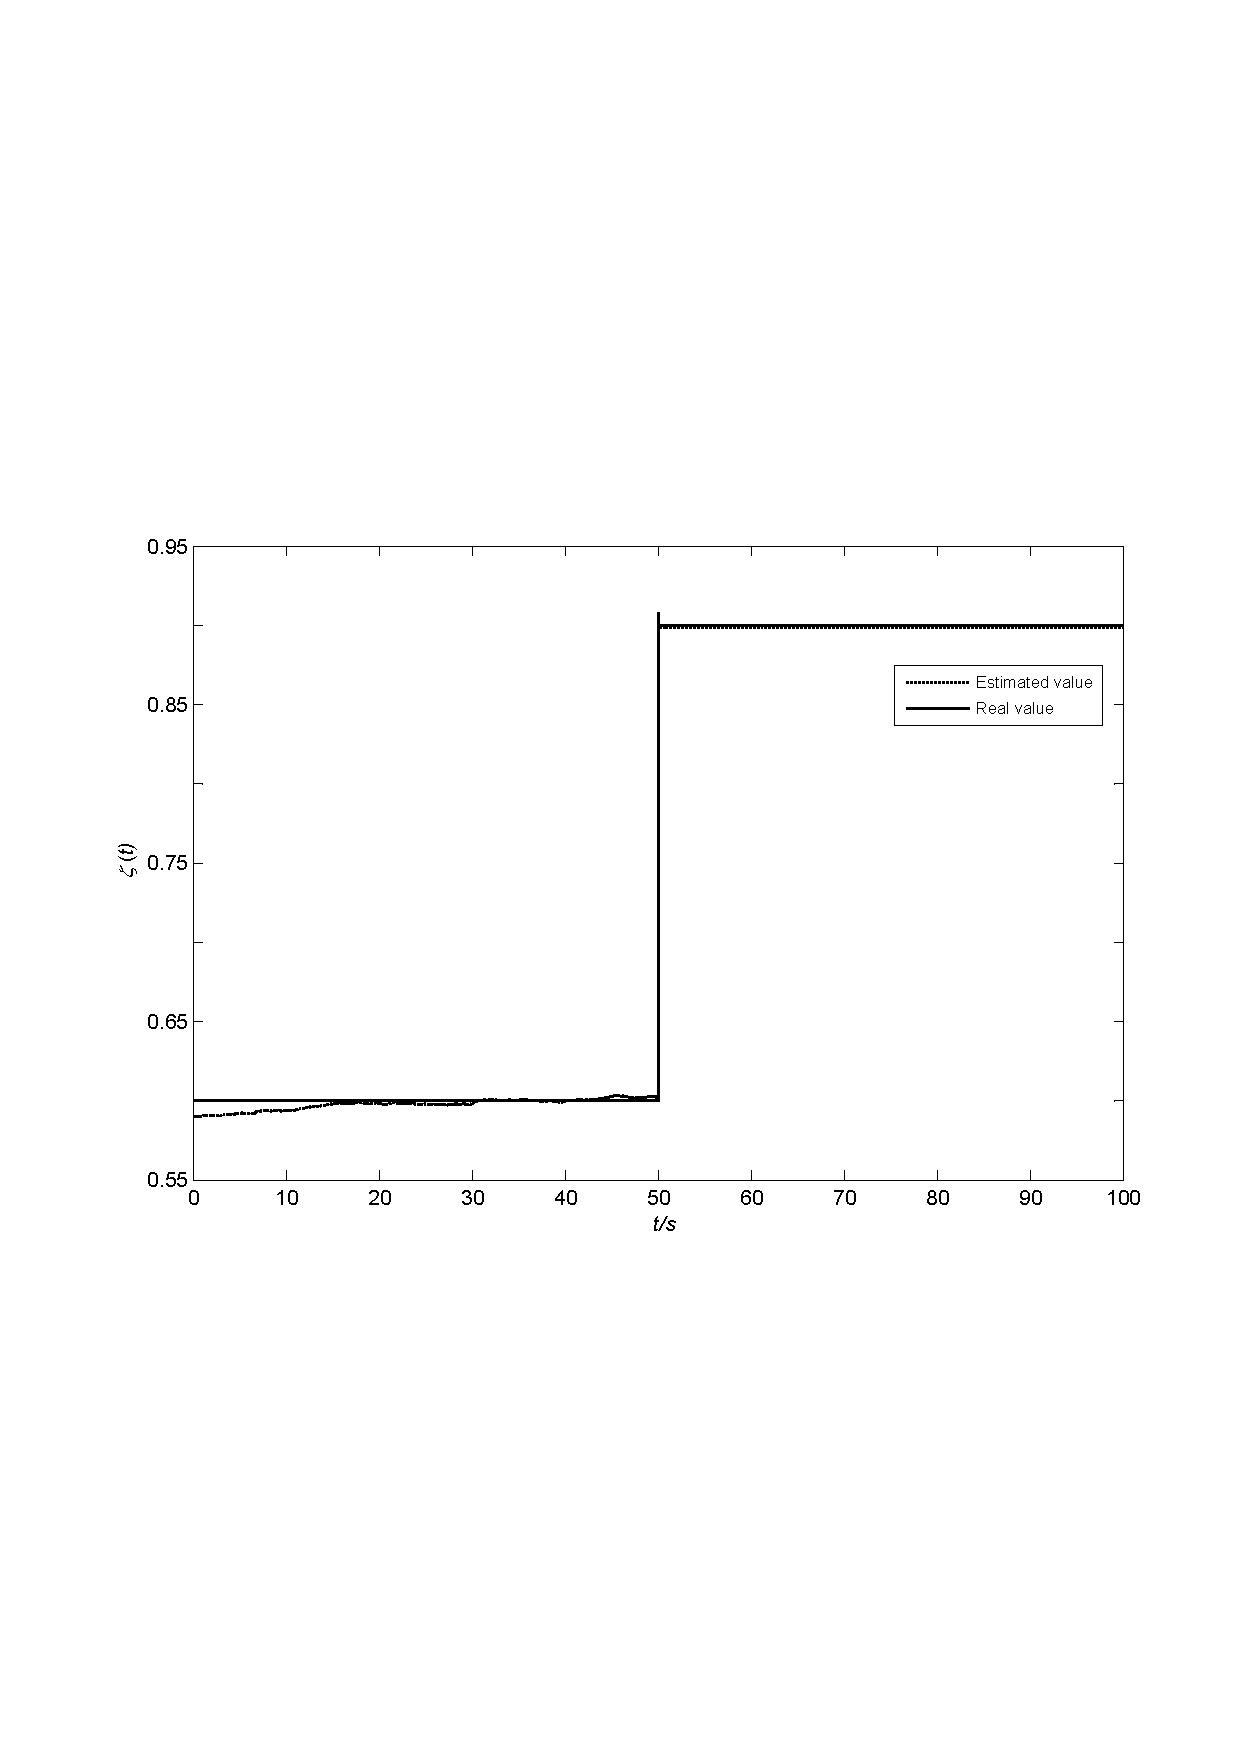
\includegraphics[width=\hsize]{fig5b.pdf}
  \caption{The parameter $\zeta_n(t)$ of hydraulic leakage}
  \label{fig:5b}
\end{figure}


\begin{figure}[!htb]
  \centering
  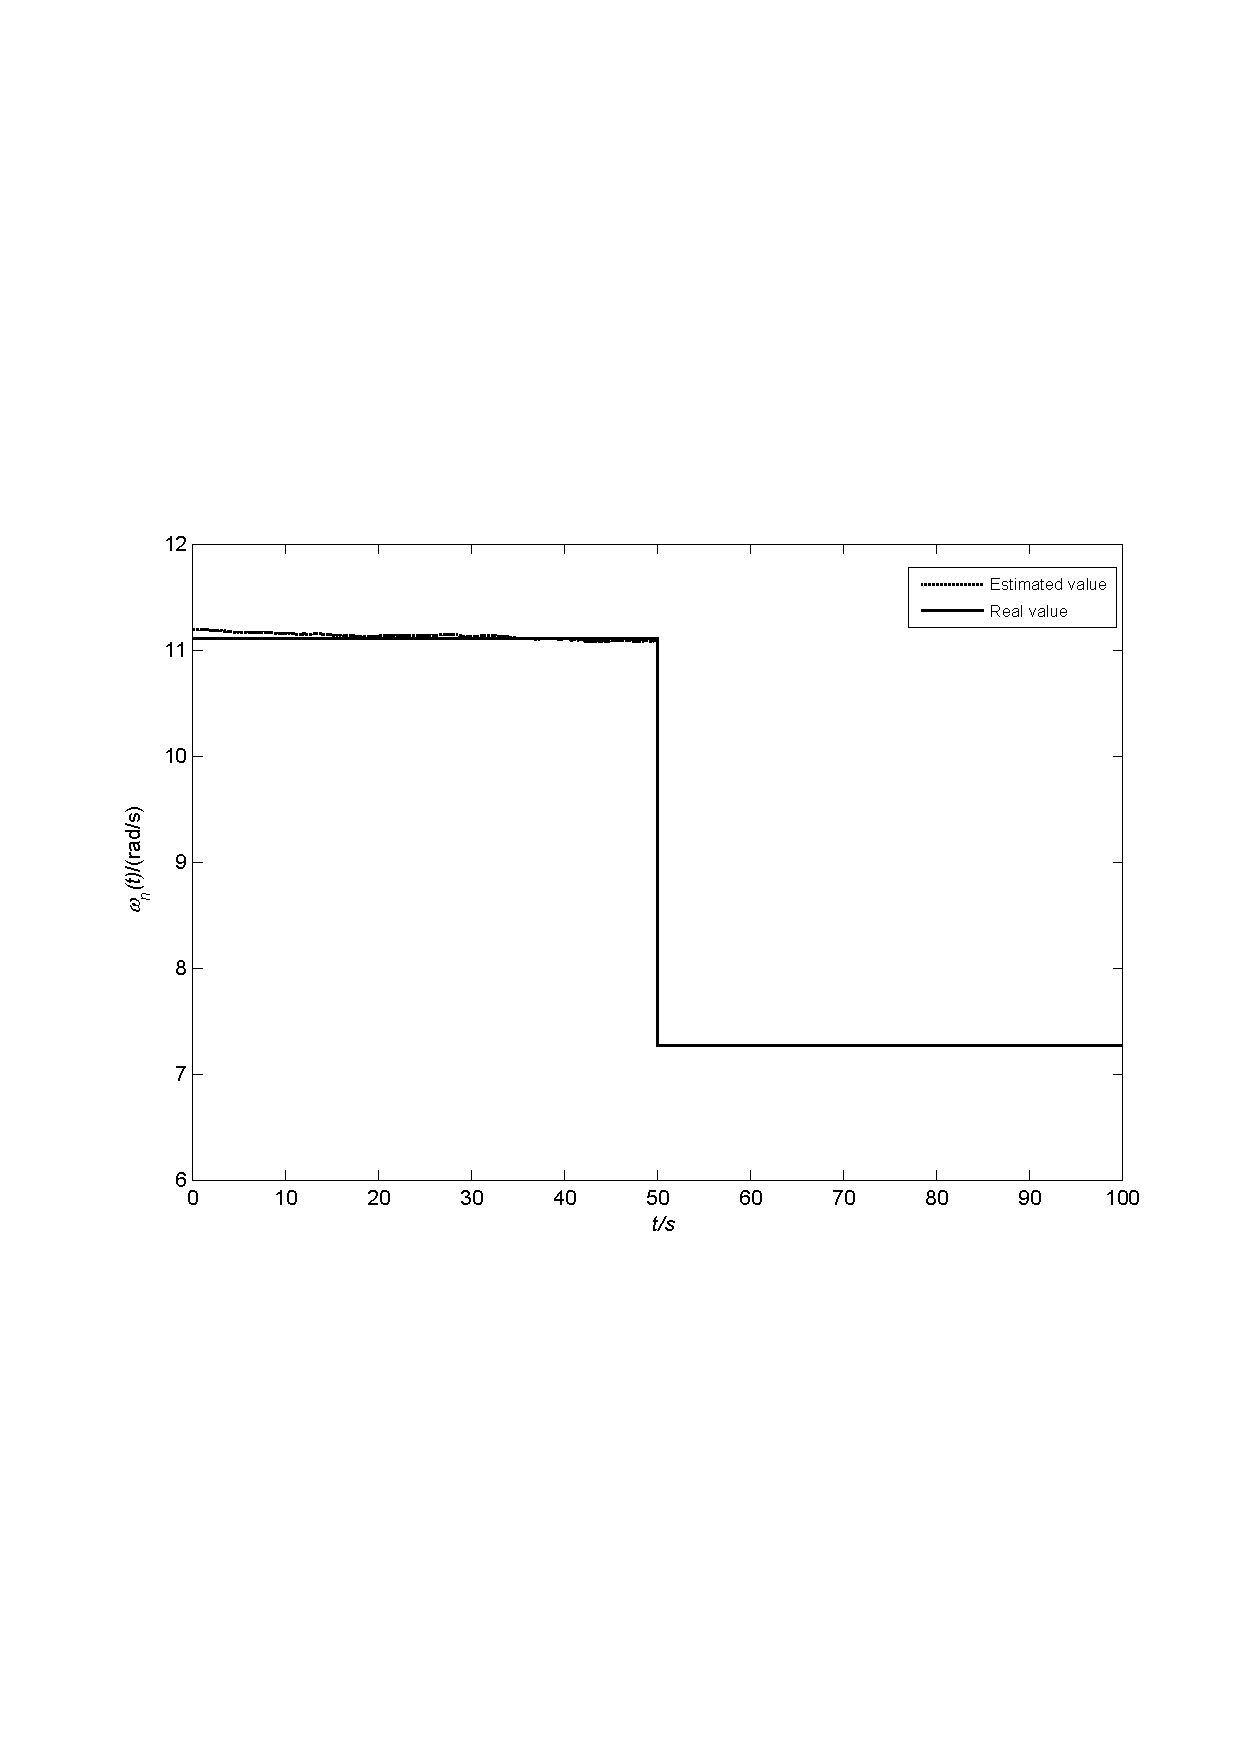
\includegraphics[width=\hsize]{fig6a.pdf}
  \caption{The parameter $\omega_n(t)$ of pump wear}
  \label{fig:6}
\end{figure}


\begin{figure}[!htb]
  \centering
  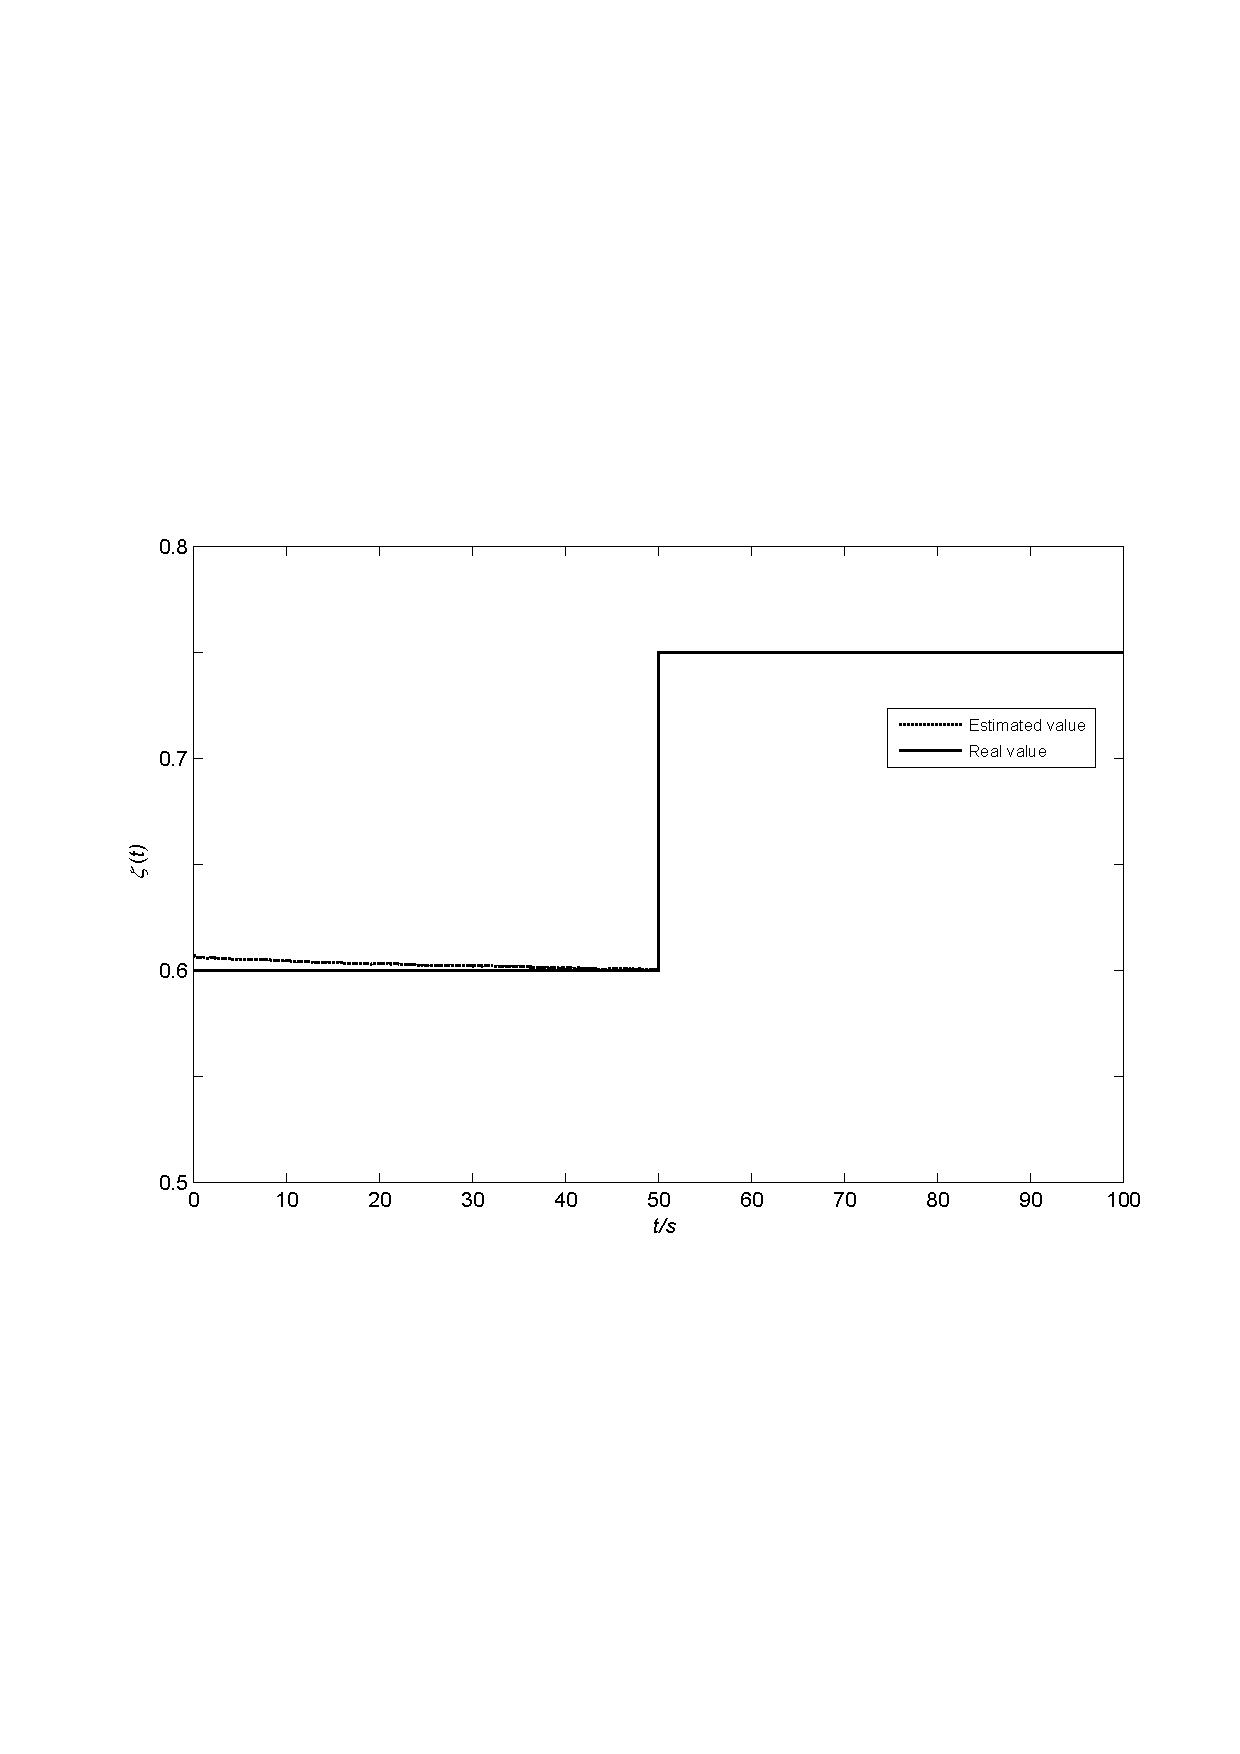
\includegraphics[width=\hsize]{fig6b.pdf}
  \caption{The parameter $\zeta_n(t)$ of pump wear}
  \label{fig:6b}
\end{figure}


\section{Simulation}

The simulation is based on the 4.8MW wind turbine benchmark model
\cite{ref:17}, the fault diagnosis system shown in Fig. \ref{fig:3},
and the VFF-RLS algorithm described in section 3.2.
When impulse invariant transformation method is used in the
discretization of the system, we can denote $u(t)=u(kT_0)=:u(k)$.
Therefore, the variable forgetting factor is $\lambda(t)=\lambda(kT_0)=:\lambda(k)$, the time-varying parameters are
$\zeta(t)=\zeta(kT_0)=:\zeta(k)$ and $\omega(t)=\omega(kT_0)=:\omega(k)$.



There are three wind turbine pitch actuator faults discussed in this
paper, which are high air content in the hydraulic oil,
hydraulic leakage and pump wear.
It is assumed that two or more faults will not occur simultaneously,
and three kinds of single fault are simulated respectively.
The parameters are shown in Tab. \ref{tab:1}.
In simulation, the fault is supposed to happen at 50s, the
fault indicator signal is
\begin{eqnarray}
  \eta_{ha}(t),\eta_{hl}(t),\eta_{pw}(t) = \left\{
  \begin{matrix}
  0, 0s\leq{}t\leq50s\\
  1, 50s<{}t\leq100s
  \end{matrix}
  \right.
\end{eqnarray}

\begin{center}
{
Table~1~~Parameters' value}\\
\label{tab:1} \vskip 3pt
\newcommand{\rb}[1]{\raisebox{1.9ex}[-2pt]{#1}}
%\renewcommand\tabcolsep{2pt}
{
\begin{tabular}{cccc}
    \hline
    Fault type                         & Value                                           \\
    \hline\hline
    No fault                           & $\omega_{n,0}=11.11rad/s, \zeta_0=0.6$          \\
    High air content in hydraulic oil  & $\omega_{n,ha}=5.73rad/s, \zeta_{ha}=0.45$      \\
    Hydraulic leakage                  & $\omega_{n,hl}=3.42rad/s, \zeta_{ha}=0.9$       \\
    Pump wear                          & $\omega_{n,pw}=7.27rad/s, \zeta_{pw}=0.75$      \\
    \hline
\end{tabular}
}
\end{center}


The parameter estimation results are shown in Fig. \ref{fig:4}
and Fig. \ref{fig:6}.


When $0s\leq{}t\leq50s$, the pitch actuator is in a stable state with
no fault, larger forgetting factor $\lambda_{max}$ is chosen for
the VFF-RLS algorithm, and the estimation error is smaller. At time
$50s$, the fault occurs, and system parameters change correspondingly.
The VFF-RLS algorithm will adjust the forgetting factor according to
Eq.(\ref{eq:27}), and smaller $\lambda(t)$ will be chosen to
ensure faster convergence speed.

When $50s<t\leq100s$, the actuator is in fault, $\lambda(t)$ changes to
$\lambda_{max}$ automatically to reduce state estimation errors.
Thus it is able to automatically adjust according to
the forgetting factor  to
meet the estimation accuracy of the steady-state and the
convergence speed of the transient moment.
Different fault types can be determined by the magnitude and
direction of the parameters' change.




\section{Conclusion}

This paper uses the system identification method for fault diagnosis of
the wind turbine hydraulic
pitch system actuator , which transmits the problem into a system
identification issue. The VFF-RLS algorithm for time-varying systems
has a high speed and precision, so parameters of the time-varying system
can be estimated. Simulation results validates feasibility and effectiveness
 of the VFF-RLS based fault diagnosis method.



%\baselineskip 5pt

%\footnotesize
\clearpage
\begin{thebibliography}{99}
\bibitem{ref:1}
Fu, Z.X.: Status and prospects on condition monitoring technologies of offshaore wind turbine. J. Control Autom. Electr. Syst. \textbf{36}(1), 121-129, (2012)


\bibitem{ref:2}
Li, S.B., Sauter, D., Aubrun, C.: Stability guaranteed active fault-tolerant control of networked control systems. J. Control Sci. Eng. \textbf{2008}(5), 22-31 (2008)


\bibitem{ref:3}
Watson, S.J., Xiang, B.J., Yang, W., Tavaner, P.J., Crabtree, C.J.: Condition monitoring of the power output of wind turbine generators using wavelets. IEEE Trans. Energy Convers. \textbf{25}(3), 715-721 (2010)


\bibitem{ref:4}
Crowther W.J., Edge K.A., Burrows C.R.: Fault diagnosis of a hydraulic actuator circuit using neural networks-an output vector space classification approach. Proceedings of the Institution of Mechanical Engineers, Part I: Journal of Systems and Control Engineering. \textbf{212}(1), 57-68, (1998)


\bibitem{ref:5}
Goharrizi A.Y., Sepehri N.: Internal leakage detection in hydraulic actuators using empirical mode decomposition and hilbert spectrum. IEEE Trans. Instrum. Meas. \textbf{61}(2), 368-378 (2012)



\bibitem{ref:6}
Goharrizi A.Y., Sepehri N.: Application of fast fourier and wavelet transforms towards actuator leakage diagnosis: a comparative study. International Journal of Fluid Power. \textbf{14}(2), 39-51 (2013)



\bibitem{ref:7}
Wu X.: Model-based and data-driven fault diagnosis for wind turbine hydraulic pitching system. Milwaukee: University of Wisconsin-Milwaukee, (2010).


\bibitem{ref:8}
Wei X., Verhaegen M.: Sensor and actuator fault diagnosis for wind turbine systems by using robust observer and filter. Wind Energy. \textbf{14}(4)  491-516 (2013)


\bibitem{ref:9}
Wu X., Li Y., Li F.: Adaptive estimation-based leakage detection for a wind turbine hydraulic pitching system. IEEE Trans. Mechatronics.  \textbf{17}(5) 907-914 (2012)


%%%%%%%%%%%%%%%%%%%%%%%%%%%%%%
\bibitem{ref:10}
Ding, F., Liu, X.P., Liu, G.: Multi-innovation least squares identification for system modeling. IEEE Trans. Syst. Man. Cybern. B. Cybern. \textbf{40}(3), 767-778 (2010)

\bibitem{ref:11}
Han, L.L, Ding, F.: Multi-innovation stochastic gradient algorithms for multi-input multi-output systems. Digit. Signal Process. \textbf{19}(4), 545-554 (2009)

\bibitem{ref:12}
Ding, F., Chen, T.: Performance analysis of multi-innovation gradient type identification methods. Automatica. \textbf{43}(1), 1-14 (2007)

\bibitem{ref:13}
Mohammadpour, J., Scherer, C.W.: Control of linear parameter varying systems with applications. Springer, (2012)

\bibitem{ref:14}
Bianchi, F.D., Battista, H.D., Mantz, R.J.: Wind Turbine Control Systems: Principle, Modeling and Gain Scheduling Design, Springer, (2007)



\bibitem{ref:15}
Odgaard, P.F., Johnson, K.E.: Wind turbine fault detection and fault tolerant control-an enhanced benchmark challenge. \emph{Proceedings of American Control Conference (ACC)}, June 17-19, 2013, Washington, America, 4447-4452.

\bibitem{ref:16}
Kolouri, S., Azimi-Sadjadi M.R., Ziemann A.: Acoustic tomography of the atmosphere using unscented Kalman filter. IEEE Trans. Geosci. Remote Sens. \textbf{52}(4), 2159-2171  (2014)

\bibitem{ref:17}
Esbensen, T., Sloth, C.: Fault diagnosis and fault-tolerant control ofwind turbines. Aalb.Univ. 16-21, 100-104 (2009)




\end{thebibliography}


\end{document}
